\documentclass[11pt]{article}
\usepackage{setspace}
\usepackage{geometry}                % See geometry.pdf to learn the layout options. There are lots.
\geometry{letterpaper}                   % ... or a4paper or a5paper or ... 
%\geometry{landscape}                % Activate for for rotated page geometry
%\usepackage[parfill]{parskip}    % Activate to begin paragraphs with an empty line rather than an indent
\usepackage{graphicx}
\usepackage{amssymb}
\usepackage{epstopdf}
\DeclareGraphicsRule{.tif}{png}{.png}{`convert #1 `dirname #1`/`basename #1 .tif`.png}

\addtolength{\topmargin}{-.75in}
% \addtolength{\oddsidemargin}{-.875in}
% \addtolength{\evensidemargin}{-.875in}
% \addtolength{\textwidth}{1.75in}

\newcommand{\toP}{\overset{p}{\to}}
\newcommand{\meanN}{\frac{1}{n}\sum_{i=1}^n}
\newcommand{\sumL}{\sum_{\ell=1}^{L_i}}
\newcommand{\meanL}{\frac{1}{L_i}\sumL}
\newcommand{\sumJ}{\sum_{j=1}^{J_i}}
\doublespacing  
\title{Using information about match quality}
\author{Rachel Anderson}
\date{\today}                                           % Activate to display a given date or no date

\begin{document}
\maketitle

\section{Estimating the mean}

\subsection{Setup}
The goal is to estimate the mean the mean of a random variable $X$ with mean $\mu$ and variance $\sigma^2$.  The econometrician observes $\{X_{i1}, X_{i2}\}_{i=1}^n$, where only one observation is drawn from the true distribution of $X$.  The other observation is noise, drawn from a distribution with mean $\kappa$ and variance $\omega^2$.      

Suppose the econometrician knows that the first observation $X_{1i}$ is drawn from the correct distribution with probability $\pi$, and drawn from the noisy distribution with probability $1-\pi$.  The two observations are perfectly dependent, so that if $X_{i1}$ is drawn from the correct distribution, then $X_{i2}$ is drawn from the incorrect distribution. 

Suppose we want to estimate a mean, $\mu =E\left[ X\right] $. For each $i$,
we have two observations, $X_{1i}$ and $X_{2i}$. One is drawn from the
correct distribution which has mean $\mu $ and variance $\sigma ^{2}$ and
one is drawn from a known incorrect distribution with \textsl{known} mean $%
\kappa $ and variance $\omega ^{2}$.

Suppose that the probability that the first is drawn from the correct
correct distribution is $\pi $. Then%
\begin{eqnarray*}
E\left[ X_{1i}\right] &=&\pi \mu +\left( 1-\pi \right) \kappa \\
E\left[ X_{2i}\right] &=&\pi \kappa +\left( 1-\pi \right) \mu
\end{eqnarray*}%
so
\begin{equation*}
E\left[ X_{1i}+X_{2i}\right] -\kappa =\pi \left( \mu +\kappa \right) +\left(
1-\pi \right) \left( \kappa +\mu \right) -\kappa =\mu
\end{equation*}%
It therefore follows that
\begin{equation*}
\frac{1}{n}\dsum\limits_{i=1}^{n}\left( X_{1i}+X_{2i}\right) -\kappa
\end{equation*}%
is a consistent estimator of $\mu $.

More generally consider an estimator of the form
\begin{equation}
\widehat{\mu }=\frac{a_{1}}{n}\dsum\limits_{i=1}^{n}X_{1i}+\frac{a_{2}}{n}%
\dsum\limits_{i=1}^{n}X_{2i}-a_{3}\kappa  \label{muhat}
\end{equation}%
Its mean would be
\begin{eqnarray}
&&E\left[ \widehat{\mu }\right] =\pi \left( a_{1}\mu +a_{2}\kappa \right)
+\left( 1-\pi \right) \left( a_{1}\kappa +a_{2}\mu \right) -a_{3}\kappa
\label{e0} \\
&=&\left( \pi a_{1}+\left( 1-\pi \right) a_{2}\right) \mu +\left( \pi
a_{2}+\left( 1-\pi \right) a_{1}-a_{3}\right) \kappa  \notag
\end{eqnarray}%
For unbiasedness, we then need%
\begin{equation}
\left( \pi a_{1}+\left( 1-\pi \right) a_{2}\right) =1  \label{e1}
\end{equation}%
or%
\begin{equation*}
a_{2}=\frac{1-\pi a_{1}}{1-\pi }=\frac{1}{1-\pi }-\frac{\pi }{1-\pi }a_{1}
\end{equation*}%
and%
\begin{equation}
\left( \pi a_{2}+\left( 1-\pi \right) a_{1}-a_{3}\right) =0  \label{e2}
\end{equation}%
The only way to do this without knowing $\pi $ is to set $a_{1}=a_{2}$. But
in that case (\ref{e2})\ inplies that $a_{1}=a_{2}=1$.

If we know $\pi $ then (\ref{e1} and (\ref{e2}) can be solved for $a_{2}$
and $a_{3}$ as a function of $a_{1}$:

\begin{center}
[here insert numerical example]
\end{center}



True p indicates the probability that $X_{1}$ is drawn from the correct distribution.  

\begin{figure}[h!]
    \centering
    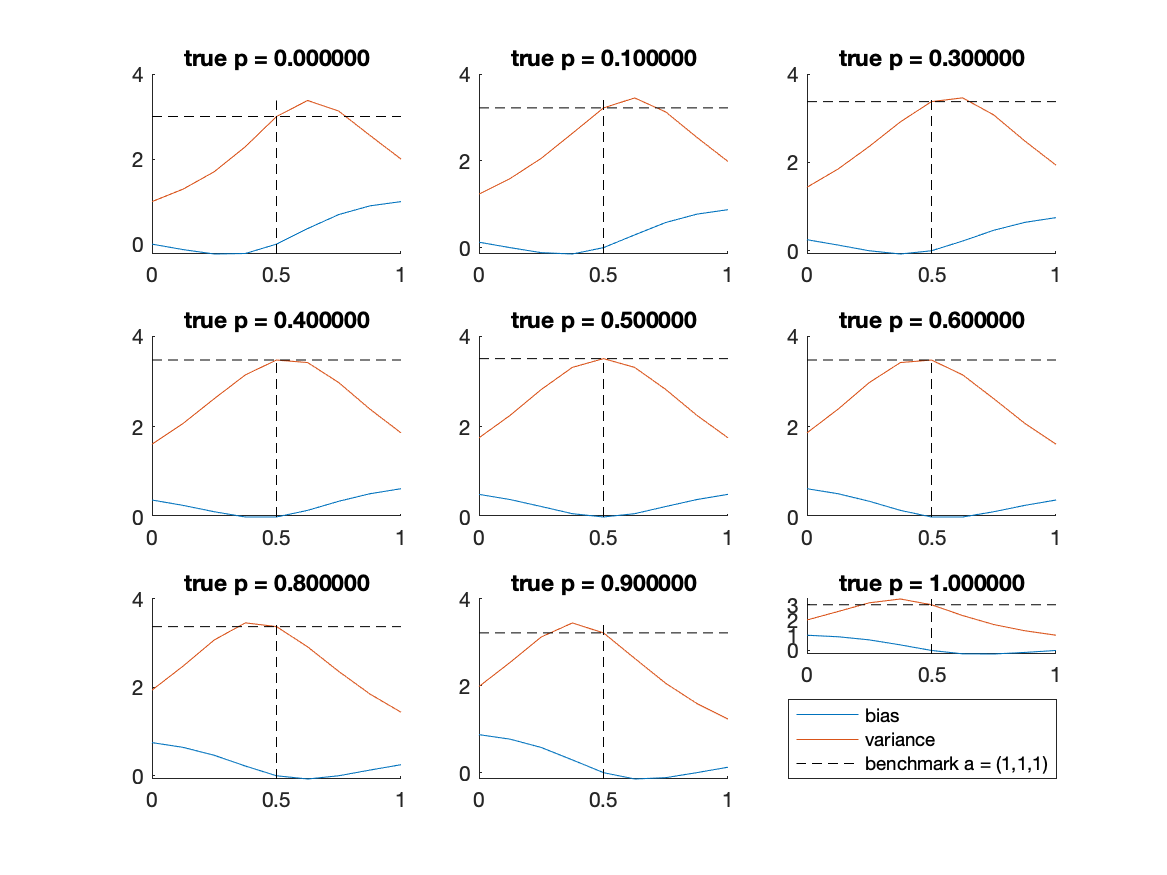
\includegraphics[width=\textwidth]{../Figures/bias_var_tradeoff_0_1_1_2.png}
    \caption{Bias-variance tradeoff implied by different beliefs about $\pi$}
    \label{fig:my_label}
\end{figure}



\subsection{Results}

The minimum variance estimator is achieved by placing all weight on the $X_{i\ell}$ with lowest variance.  The bias function is quadratic in $\pi$, with zeros achieved at $\hat{\pi}=\pi_0$ and $\hat{\pi}=0.5$.  The minimum MSE estimator depends on the choice of correct and incorrect distributions. 

With two observations, everything is symmetric so we only need to look at values between 0 and 0.5.


\end{document}  